%&latex
\documentclass[10pt,fleqn]{article} 

\pdfoutput=1

\addtolength{\oddsidemargin}{-.875in}
\addtolength{\evensidemargin}{-.875in} \addtolength{\textwidth}{1.75in}

\addtolength{\topmargin}{-.875in} \addtolength{\textheight}{1.75in}

\openup 1em

%macro for commenting
\usepackage{color}

\newcommand{\leo}[1]{{\color{blue}{#1}}}
\newcommand{\alex}[1]{{\color{red}{Alex: #1}}}

% \newcommand{\Xbeta}{ X_i \theta}
\newcommand{\xbeta}{ x_i \beta} \newcommand{\xtheta}{ x_i \theta}
% \newcommand{\xbetaij}{ x_{ij}^T \theta}
\newcommand{\sgamma}{s_{ij}^T\gamma_i} \newcommand{\core}{\textbf{CORE}}

\usepackage[round]{natbib}

\usepackage{rotating} \usepackage{graphicx} \usepackage{subcaption}

\usepackage{float} \usepackage{bbm}

\usepackage{amsthm,amsmath, amssymb} \usepackage{mathrsfs}
\usepackage{subcaption}
\usepackage[normalem]{ulem}
%\usepackage{nicefrac}

%\usepackage{pgfplots}
%\pgfplotsset{compat=1.8}
%\usepackage{mathtools}
\usepackage{tikz}

\newtheorem{theorem}{Theorem} \newtheorem{lemma}{Lemma}
\newtheorem{corollary}{Corollary} \newtheorem{remark}{Remark}
\newtheorem{example}{Example} \newtheorem*{Hausdorff_def}{Definition -
Hausdorff Measure}


\usepackage{algorithm} \usepackage{algpseudocode} \usepackage{array}

%\usepackage{mhequ}
\newcommand{\be}{\begin{equation}\begin{aligned} }
\newcommand{\ee}{\end{aligned}\end{equation} }
\newcommand{\bb}[1]{\mathbb{#1}} \newcommand{\mc}[1]{\mathcal{#1}}
\DeclareMathOperator{\Binom}{Binomial} \DeclareMathOperator{\No}{No}
\DeclareMathOperator{\PG}{PG} \DeclareMathOperator{\IG}{Inverse-Gamma}
\DeclareMathOperator{\Ga}{Gamma} \DeclareMathOperator{\Bern}{Bernoulli}
\DeclareMathOperator{\U}{Uniform} \DeclareMathOperator{\Poi}{Poisson}
\DeclareMathOperator{\NB}{NB} \DeclareMathOperator{\cov}{cov}
\DeclareMathOperator{\var}{var} \DeclareMathOperator{\diag}{diag}
\DeclareMathOperator{\Diag}{Diag}
\newcommand{\KL}[2]{\textnormal{KL}\left(#1 \parallel #2\right)}
\DeclareMathOperator{\1}{\mathbbm{1}} \DeclareMathOperator{\bigO}{\mc O}
\newcommand{\dt}{\epsilon} % Stepsize of leapfrog
\newcommand{\mass}{M} %Mass matrix 
\newcommand{\hess}{\mathbf{H}} % Hessian notation.



\thispagestyle{empty} \baselineskip=28pt

\title{\textbf{Bayesian constraint relaxation}}

\author{Leo L Duan, Alexander L Young, Akihiko Nishimura, David B Dunson} 

\date{}
\begin{document}

\maketitle % {\bf Abstract:}

Prior information often takes  the form of parameter constraints. Bayesian
methods include such information through prior distributions having constrained
support. By using posterior sampling algorithms, one can quantify uncertainty
without relying on asymptotic approximations. However, {\em sharply}
constrained priors are (a) unrealistic in many settings; and (b) tend to limit
modeling scope to a narrow set of distributions that are tractable computationally.
We propose to solve both of these problems via a general class of Bayesian 
{\em constraint relaxation} methods.  The key idea is to replace the sharp
indicator function of the constraint holding with an exponential kernel.  This
kernel decays with distance from the constrained space at a rate depending on 
a relaxation hyperparameter.  By avoiding the sharp constraint, we enable use of
off-the-shelf posterior sampling algorithms, such as Hamiltonian Monte Carlo, 
facilitating automatic computation in broad models. We study the constrained and 
relaxed distributions under multiple settings, and theoretically quantify their 
differences. We illustrate the method through multiple novel modeling examples.

\vskip 12pt
        %\baselineskip=12pt \par\vfill\noindent
        {\noindent KEY WORDS: Constrained Bayes, Constraint
        functions, Shrinkage on Manifold, Support Expansion, Ordered Simplex}
%\par\medskip\noindent \clearpage\pagebreak\newpage
\pagenumbering{arabic}

\newpage



\section{Constraint Relaxation Methodology}

Assume that $\theta \in \mathcal{D} \subset \mathcal{R}$ is an unknown parameter, 
with $\dim(\mathcal{R})=r < \infty$.  The constrained sample space $\mathcal{D}$ is 
embedded in the $r$-dimensional Euclidean space $\mathcal{R}$, and can have 
either zero or positive measure with respect to Lesbesgue measure on $\mathcal{R}$.  

The traditional Bayesian approach to including constraints requires a
prior density $\pi_\mathcal{D}(\theta)$ with support on $\mc D$. The posterior density of $\theta$
given data $Y$ and $\theta \in \mathcal{D}$ is then
\begin{eqnarray}
\pi_{\mc D}(\theta \mid  Y) % & = & \frac{ \pi_\mathcal{D}(\theta)\mathcal{L}(\theta; Y) }{
%\int_{\mc D} \pi_\mathcal{D}(\theta)\mathcal{L}(\theta; Y)d\theta } 
& \propto & \pi_\mathcal{D}(\theta)\mathcal{L}(\theta; Y). \label{eq:sharp}
\end{eqnarray}
We assume in the sequel that the restricted prior $\pi_\mathcal{D}(\theta) \propto 
\pi_{\mc R}(\theta)\mathbbm{1}_{\mc D}(\theta)$, with $\pi_{\mc R}(\theta)\mathbbm{1}_{\mc D}(\theta)$
an initial unconstrained prior on ${\mc R}$ and $\mathbbm{1}_{\mc D}(\theta)$ an indicator
function that the constraint is satisfied.

As noted in Section 1, there are two primary problems motivating this article.  The first is that it is often
too restrictive to assume that $\theta$ is {\em exactly} within ${\mc D}$ {\em a priori}, and often is more plausible to assume that $\theta$ has high probability of falling within a small neighborhood of ${\mc D}$.
The second is that the difficulty of posterior sampling from (\ref{eq:sharp}) has greatly limited the scope of modeling, and there is a critical need for general algorithms that are tractable for a broad variety of choices of prior, likelihood and constraint.

In attempting to address these problems, we propose to replace (\ref{eq:sharp}) with the following {\em COnstraint RElaxed} (CORE) posterior density: 
\begin{equation}
\label{EQ:Rel_Dens_Motivation}
\tilde{\pi}_{\lambda}(\theta) \propto
\mathcal{L}(\theta; Y)  \pi_\mathcal{R}(\theta)
\exp\bigg(-\frac{1}{\lambda} \|v_\mathcal{D}(\theta)\|\bigg),
\end{equation}
where we repress the conditioning on data $Y$ in $\tilde{\pi}_{\lambda}(\theta)$ for concise notation. \leo{$\pi_{\mc R}(\theta)$ is
a density related to (often, proportional to) $\pi_\mathcal{D}(\theta)$,  except with a different support.}
  We assume the the initial prior $\pi_{\mc R}(\theta)$ is proper, and use $\|v_\mathcal{D}(\theta)\|$ as
a distance from $\theta$ to the constrained space.  For example, $\|v_\mathcal{D}(\theta)\| = \inf_{x\in\mathcal{D}} \|\theta-x\|_2$ with $\|.\|$ an appropriate metric.

The hyperparameter $\lambda > 0$ controls how concentrated the prior is around 
${\mc D}$, and as $\lambda \to 0$ the kernel $\exp\big(- \lambda^{-1}\|v_\mathcal{D}(\theta)\|)$
converges to $\mathbbm{1}_\mathcal{D}(\theta)$ in a pointwise manner, excluding $\theta \in \partial {\mc D}$ on the boundary of ${\mc D}$.  For all $\lambda > 0$, $\tilde{\pi}(\theta)$ has 
support $\mathcal{R}$.  This unrestricted support greatly simplifies the design of 
posterior sampling algorithms, making it easier to consider a much wider
variety of models.

In this article, we assume $\theta$ is a continuous random variable with $\pi_{\mc R}(\theta)$
absolutely continuous with respect to Lebesgue measure $\mu_\mathcal{R}$ on $\mathcal{R}$. To construct a relaxed distribution, we first start by considering a $d$-neighborhood of ${\mc D}$
$$\{\theta\in \mc R: \|v_\mathcal{D}(\theta)\| \le d) \}.$$
Clearly, the definition of distance $\|v_\mathcal{D}(\theta)\|$ is critical as it describes how support expansion occurs around $\mc D$. We elaborate the details in the next section.

\subsection{Distance to Constrained Space}

To induce a neighborhood surrounding only $\mc D$, a minimal condition is that $\|v_{\mc D}(\theta)\|$ is zero for $\theta \in \mathcal{D}$ and positive for $\theta\not\in\mathcal{D}$. There are many choices of distances that satisfy this condition; however, for two useful purposes, one may be interested in one of the distances.

(I) The ones directly measuring how far $\theta \in \mc R$ is from the original constrained space $\mc D$. This is useful when one hopes to directly control and/or measure the support expansion based on $\theta$. For example, when $\mc D$ is a symmetric compact manifold, one might be interested in uniformly expanding the support of $\theta$, so that the relaxation does not create any directional asymmetry. In this article, we consider a simple isotropic distance

\begin{eqnarray}
\|v_{\mc D}(\theta)\| = \inf_{x\in\mathcal{D}} \|\theta-x\|_k,
\end{eqnarray}
where $\|\cdot\|_k$ denotes a $k$-norm distance, commonly $k=1$ or $2$.

(II) The ones measuring how far a function of $\theta \in \mc R$ is from the constrained value when $\theta\in \mc D$. This is particularly useful when the interest of relaxation is not on parameter $\theta$, but on the function $f(\theta)$\ associated with the constraint. For example, when a model is constrained by assigning an inequality to a function, one may be interested in how much the function deviates from the constrained value. Similar to (i), we also consider a simple distance

\begin{eqnarray}
\|v_{\mc D}(\theta)\| = \inf_{x\in\mathcal{D}} \|f(\theta)-f(x)\|_k.
\end{eqnarray}
This distance has a simple closed form, when $f(x)$ is a constant for $\theta\in \mc D$.

To illustrate their difference, we consider a simple constrained space $\mc D=\{(\theta_1,\theta_2):  \theta_1 >0, \theta_2>0, \theta_1+\theta_2<1\}$. For type-I distance, we use $2$-norm $\inf_{x\in\mathcal{D}} \|\theta-x\|_{2}$ around space $\mc D$. One function of interest is the total violation to the three inequalities $f((\theta))= (-\theta_1)_+ + (-\theta_2)_+ + (1-\theta_1-\theta_2)_+$ where $(x)_+ = x$ if $x>0$ and $0$ otherwise. As $f(\theta)=0$ when $\theta\in \mc D$, the associated type-II distance is simply
$\|v_{\mc D}(\theta)\| =f (\theta)$. Figure~\ref{fig:two_distances}
plots the expanded space of $\{\theta: \|v_{\mc D}(\theta)\|< 0.1\}$ and the values of $f(\theta)$ along $\|v_{\mc D}(\theta)\| = 0.1$, using those
two distances.


\begin{figure}[H]
% type 1 distance
    \begin{subfigure}[b]{0.45\textwidth}
        \centering
        \resizebox{\linewidth}{!}{
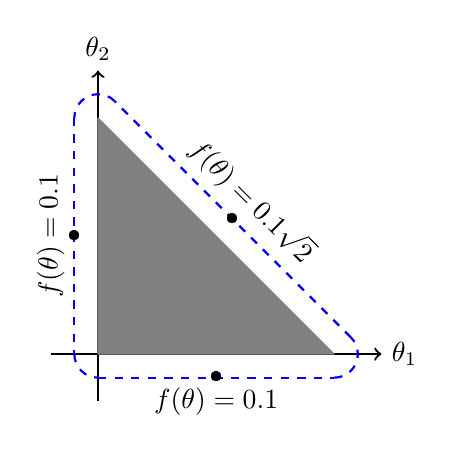
\begin{tikzpicture}[scale=3, line join=bevel]

\draw[help lines, color=gray!30, dashed] (-0.2,-0.2) grid (0.1,0.1);
\draw[->, thick] (-0.2,0)--(1.2,0) node[right]{$\theta_1$};
\draw[->, thick] (0,-0.2)--(0,1.2) node[above]{$\theta_2$};


\draw[gray, thin, fill = gray] (0,0) -- (1,0) -- (0,1) -- cycle;
\draw[blue, thick, dashed] (-0.1,1) -- (-0.1,0);
\draw[blue, thick, dashed] (-0.1,0) arc (180:270:0.1);
\draw[blue, thick, dashed] (0,-0.1) -- (1,-0.1);
\draw[blue, thick, dashed] (1,-0.1) arc (-90:45:0.1);
\draw[blue, thick, dashed] (1.0707, 0.0707) --  (0.0707,1.0707); 
\draw[blue, thick, dashed] (0.0707,1.0707) arc (45:180:0.1);

\draw (-0.1,0.5) node[] {\textbullet};
\draw (0.5, -0.1) node[] {\textbullet};
\draw (0.57,0.57) node[] {\textbullet};

\node[rotate=90] at (-0.2,0.5) {$f(\theta)=0.1$};
\node[rotate=0] at (0.5,-0.2) {$f(\theta)=0.1 $};
\node[rotate=-45] at (0.65,0.65) {$f(\theta)=0.1 \sqrt{2}$};
\end{tikzpicture}
        }
        \caption{Expanded support using type-I distance}
    \end{subfigure}
% type 2 distance
\begin{subfigure}[b]{0.45\textwidth}
        \centering
        \resizebox{\linewidth}{!}{
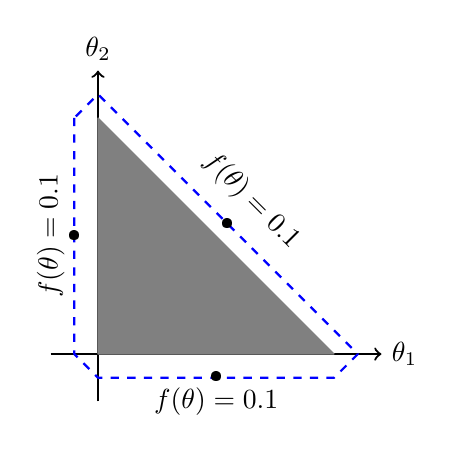
\begin{tikzpicture}[scale=3, line join=bevel]

\draw[help lines, color=gray!30, dashed] (-0.2,-0.2) grid (0.1,0.1);
\draw[->, thick] (-0.2,0)--(1.2,0) node[right]{$\theta_1$};
\draw[->, thick] (0,-0.2)--(0,1.2) node[above]{$\theta_2$};

\draw[gray, thin, fill =gray] (0,0) -- (1,0) -- (0,1) -- cycle;

\draw[blue, thick, dashed] (-0.1,1) -- (-0.1,0) --
 (-0.1,0) -- (0,-0.1)--
  (0,-0.1) -- (1,-0.1)-- 
  (1.1, 0) --  (0,1.1)  -- cycle;; 


\draw (-0.1,0.5) node[] {\textbullet};
\draw (0.5, -0.1) node[] {\textbullet};
\draw (0.55,0.55) node[] {\textbullet};

\node[rotate=90] at (-0.2,0.5) {$f(\theta)=0.1$};
\node[rotate=0] at (0.5,-0.2) {$f(\theta)=0.1$};
\node[rotate=-45] at (0.65,0.65) {$f(\theta)=0.1$};


\end{tikzpicture}}
        \caption{Expanded support using type-II distance}
    \end{subfigure}

 \caption{ The boundary (blue dashed line) along $\|v_{\mc D}(\theta)\| = 0.1$  formed by two type of distances, around a space formed by three inequalities (gray area) \label{fig:two_distances}. Panel(a) shows type-I distance uniformly expands
the support of the $\theta$; panel (b) shows type-II distance, while does
not uniformly expands the support, retains the same amount of total violation
 to constraints (quantified in a function $f(\theta)$) along the boundary.}
\end{figure}




\subsection{Constraint Relaxation}
Intuitively, the exactly constrained model can be viewed as the result of fixing the distance $\|v_\mathcal{D}(\theta)\| = 0$.  one could achieve constraint relaxation by assigning
a distribution that allows $\|v_\mathcal{D}(\theta)\|$ to be slightly greater than $0$. However, this raises two important questions:
(i) how are the  constrained density and
relaxed density related to each other? (ii) what are
the limiting conditions that apply to this methodology?
It turns out the answers are very different depending
on whether the constrained space $\mc D$ has a zero
measure with respect to $\mu_{\mc R}$. Therefore, we
discuss them separately in the next two subsections.

\subsubsection{Constrained Space with Positive Measure}


We start with
the case when $\mathcal{D}$ is a subset of $\mc R$ with positive measure with respect to a unconstrained
density $\pi_{\mc R}(\theta)$, that is $\mu_\mathcal{R}(\mc D)>0$.
  Some common examples include linear inequality constraints $a^T\theta < 0$ or non-linear inequality constraints.  The sharply constrained prior is simply a space-truncated version of the unconstrained prior 
$\pi_{\mc R}(\theta)$, leading to the posterior density
$$\pi_\mathcal{D}(\theta\mid Y) = \frac{\mathcal{L}(\theta; Y)
\pi_\mathcal{R}(\theta)\mathbbm{1}_\mathcal{D}(\theta)}{\int_\mathcal{D}
\mathcal{L}(\theta; Y)
\pi_\mathcal{R}(\theta)d\mu_\mathcal{R}(\theta)}\propto \mathcal{L}(\theta;
Y) \pi_\mathcal{R}(\theta)\mathbbm{1}_\mathcal{D}(\theta), $$
which is defined with respect to $\mu_\mathcal{R}$. 

For constraint relaxation, one could simply replace
the indicator  with the exponential function
\begin{equation}
\label{EQ:relaxedDensityPosMeasure}
\tilde{\pi}_\lambda(\theta \mid Y) =
\frac{\mathcal{L}(\theta;
Y)\pi_\mathcal{R}(\theta)\exp\big(-
\lambda^{-1}{\|v_{\mc
D}(\theta)\|}\big)}{\int_{\mathcal{R}}\mathcal{L}(\theta; Y)
\pi_\mathcal{R}(\theta)\exp\big(-{\lambda^{-1}}{\|v_{\mc
D}(\theta)\|}\big)
d\mu_\mathcal{R}(\theta)} \propto
\mathcal{L}(\theta; Y)
\pi_\mathcal{R}(\theta)\exp\big(-{\lambda^{-1}}{\|v_{\mc
D}(\theta)\|}\big)
\end{equation}
which is also absolutely continuous with respect to $\mu_\mathcal{R} $. 

The exponential function can be view as part of a folded Laplace kernel
$$\frac{1}{\lambda}\exp(-\frac{w}{\lambda})$$
 for random variable $w=\|v_{\mc D}(\theta) \|$ with scale $\lambda$. Laplace enjoys sharp sharp concentration near zero with small $\lambda$ and is routinely used in shrinkage literature. This is useful when one wants to allow only a small relaxation from $\|v_{\mc D}(\theta) \|=0$ with a fixed small $\lambda$, or apply shrinkage towards a constrained space by estimating $\lambda$ posteriori. Naturally, one could consider other kernel such as folded generalized Pareto (REFS). In this article, we focus on the folded Laplace case for its simplicity.

To address the two motivating questions at the beginning, provided $\|v(\theta)\|=0$ if and only if $\theta\in \mc D$, the constrained density is obviously the pointwise limit of relaxed density when $\lambda\to 0$, and this relaxation method is generally applicable with little restriction.
   
As shown in the last section, the choice of distance has an impact on the geometry of the posterior support. Therefore, care must be taken to ensure the choice is coherent with the prior belief. In the previous example of triangular constrained region, assuming $\pi_\mc R(\theta)$ is a uniform density over a compact $\mc R$, choosing type-I distance reflects the belief that the parameter $\theta$ can depart from $\mc D$ at equal distance with same prior probability; choosing type-II distance reflects the belief that the prior probability would drop at a rate depending on the total violation to inequalities. On the other hand, if $\lambda$ is arbitrarily small, their difference  vanishes, we will quantify this behavior in the theory section.

For now, we illustrate a Gaussian with a relaxed inequality. Suppose $\theta$ is the normal mean of the data, with the prior of $\theta$ follows a weakly informative Gaussian
 $$y_i \stackrel{iid}{\sim} \No(\theta,1) \text{ for } i =1,\ldots,n, \qquad \theta \sim\No(0, 1000)$$ 
 with an prior belief of inequality $\theta<1$. The posterior under a sharply constrained model is

$$ \pi_{\mc D}(\theta \mid Y) \propto {\sigma^{-1}}\phi(\frac{\theta- \mu}{\sigma}) \mathbbm{1}_{\theta<1}, \quad \mu=    \frac{ \bar yn}{ 1/1000 + n },   \quad \sigma^2 = \frac{1}{ 1/1000 + n },$$
where $\phi$ denotes the density of standard Gaussian. 
However, suppose the average data $\bar y=1.2$ and let $n$ grow. The posterior become increasingly concentrated on the boundary and the sharp inequality becomes much less plausible (Figure~\ref{fig:gaussian_inequality}(a)). In contrast, consider the posterior under relaxed constraint:

$$ \pi_{\lambda}(\theta \mid Y) \propto {\sigma^{-1}}\phi(\frac{\theta- \mu}{\sigma}) \exp(-\frac{(\theta-1)_+ }{\lambda}) , \quad \mu=    \frac{ \bar y n}{ 1/1000 + n },   \quad \sigma^2 = \frac{1}{ 1/1000 + n }$$
where $(\theta-1)_+$ is the type-I distance to constrained space. With $\lambda=10^{-2}$, at $n=10$ and $100$, the relaxed posteriors are similar to the sharply constrained
ones; however, $\bar y=1.2$ with a large sample size $n=1000$ leads to result that show the true mean is
very likely outside the presumed constrained region.

\begin{figure}[H]
\begin{subfigure}[b]{0.45\textwidth}
 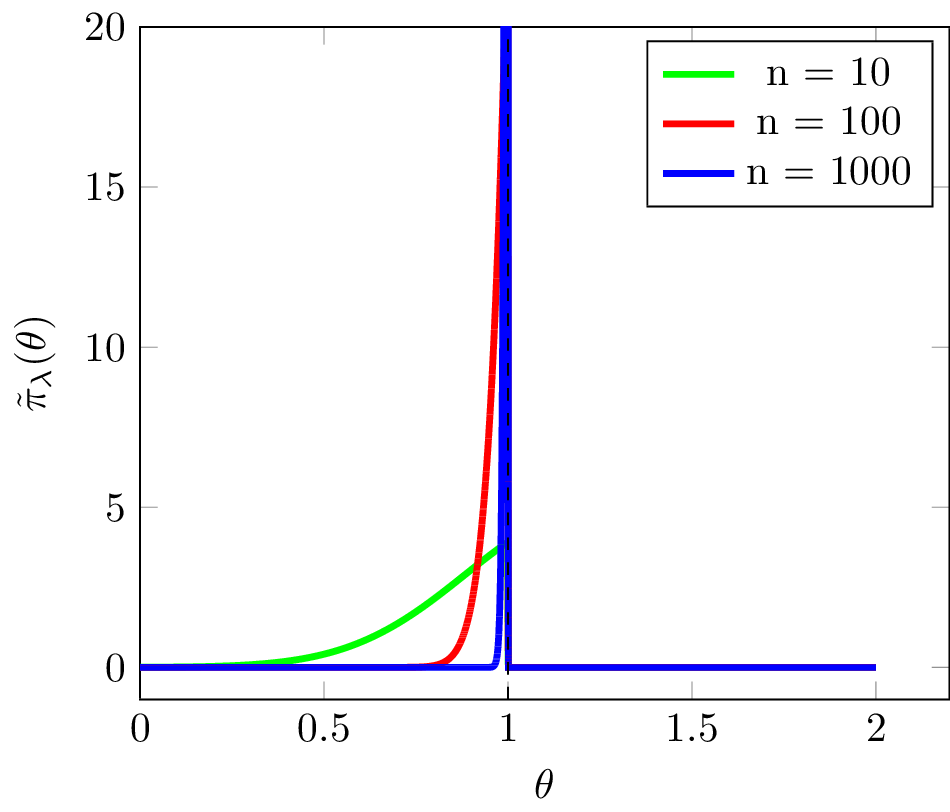
\includegraphics[width=1\textwidth]{gaussianInequalitySharp.png}
 \caption{Sharply constrained posterior}
\end{subfigure}
\begin{subfigure}[b]{0.45\textwidth}
 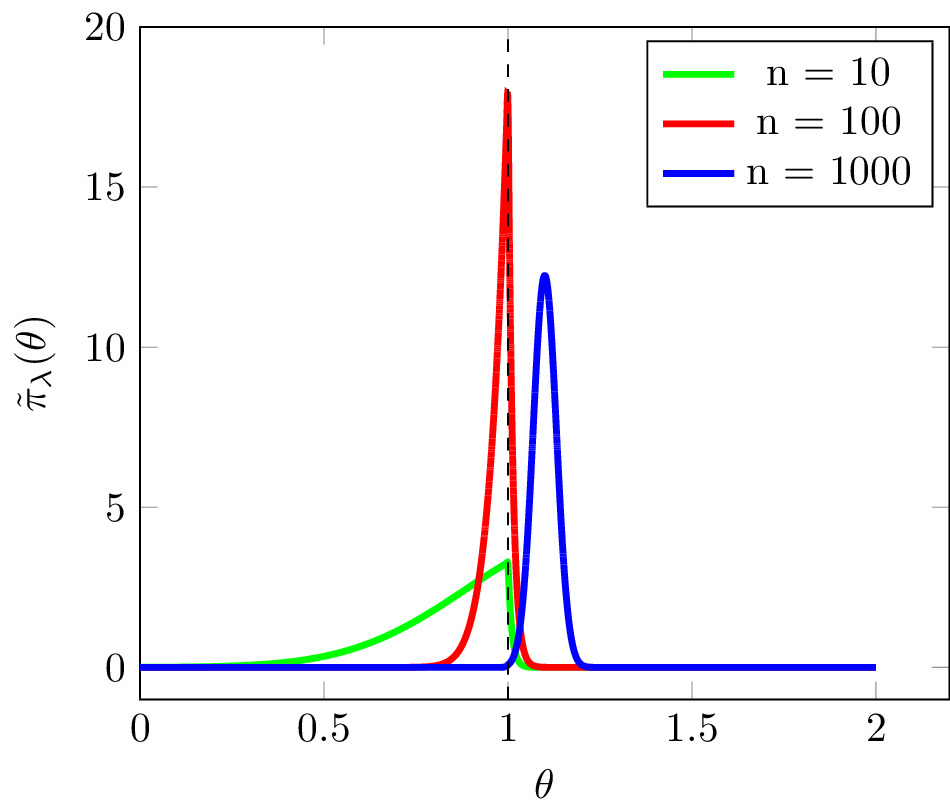
\includegraphics[width=1\textwidth]{gaussianInequalityRelaxed.png}
 \caption{Constraint relaxed posterior}
\end{subfigure}
 \caption{Density of posteriors for Gaussian mean under sharp and relaxed constraints. The relaxed constraint allow strong evidence of large
 sample with mean $\bar y=1.2$ to overpower the constraint,
  generating estimated
 mean outside the constrained region.  \label{fig:gaussian_inequality}}
\end{figure}



\subsection{Constrained Space with Zero Measure}
\label{SEC:Zero_Measure_Methods}

In the second case, we consider when $\mathcal{D}$
is a measure zero subset of $\mathcal{R}$, i.e.
$\int_\mathcal{D}\mathcal{L}(\theta;Y)\pi_\mathcal{R}(\theta)d\mu_\mathcal{R}(\theta)=0$.
Recall that $\mathcal{R}$ have dimensionality $r$, we now restrict
ourselves to the setting where $\mathcal{D}$ can be represented implicitly
as the solution set of a consistent system of equations $\{v_j(\theta) =
0\}_{j=1}^s$, so that $\mathcal{D} =\{\theta \mid v_j(\theta) =0, \, j =
1, \dots,s\}$ is a $(r-s)$-dimensional submanifold of $\mc R$.  While we
impose some restrictions, the result applies on many common constraints (e.g.
$\sum_i \theta_i = 1$, $\theta^T\theta=I$).

Due to the zero measure, one cannot obtain
conditional probability as before by simply re-normalizing
$\big[\int_\mathcal{D}\mathcal{L}(\theta;Y)\pi_\mathcal{R}d\mu_\mathcal{R}(\theta)\big]^{-1}.$
Instead, we resort to the generalized definition of conditional
probability, named \emph{regular conditional probability} (r.c.p.)
\citep{kolmogorov1950foundations} to derive a constrained density coherent
with $\pi_\mathcal{R}.$

More technical definition of the r.c.p. is provided in the appendix. For
now, the following intuition is sufficient. While $\mathcal{D}$ has zero
$r$-dimensional volume (i.e. zero Lebesgue measure), it has a positive
$(r-s)$-dimensional `surface area', formally known as normalized Hausdorff
measure, denoted by $\bar{\mathcal{H}}^{(r-s)}$ . We can use it as the
normalizing constant to obtain a r.c.p density:

$$\pi_{\mc D}(\theta \mid Y) = \dfrac{
{\mathcal{L}(\theta;Y)\pi_\mathcal{R}(\theta)}{J^{-1}(\nu_\mathcal{D}(\theta))
\mathbbm{1}_{\mc D}(\theta)
}
} {\int_\mathcal{D}
{\mathcal{L}(\theta;Y)\pi_\mathcal{R}(\theta)}{J^{-1}(\nu_\mathcal{D}(\theta))}
d\bar{\mathcal{H}}^{(r-s)}(\theta)} \propto
{\mathcal{L}(\theta;Y)\pi_\mathcal{R}(\theta)}{J^{-1}(\nu_\mathcal{D}(\theta))
\mathbbm{1}_{\mc D}(\theta)
}.
$$
where $J(\nu_\mathcal{D}(\theta)) =
\sqrt{(D\nu_\mathcal{D})'(D\nu_\mathcal{D})}$ is the Jacobian
of $\nu_\mathcal{D}$, which we assume is positive. This term is
introduced as we fix $\{v_j(\theta)=0\}_{j=1}^{s}$.  The density is
defined with respect to $\bar{\mathcal{H}}^{(r-s)}$.

Similar to the constrained space with positive measure, we face the
same modeling and computing challenges here as well.  Additionally,
although Hausdorff measure is a standard tool in geometric measure theory
\citep{federer2014geometric}, the available distributions are scarce in
Bayesian literature.

We now take a similar strategy by considering $\|\nu_\mathcal{D}(\theta)\|$ as
the distance from $\theta$ to $\mathcal{D}.$ Thus, $\|v_\mathcal{D}(\theta)\| =
0$ implies that $\theta \in \mathcal{D}$, otherwise
$\|v_\mathcal{D}(\theta)\|_1 >0$ implies $\theta\notin\mathcal{D}.$
To construct a relaxed density, we expand support in the neighborhood of
$\{\theta:\|v_{\mc D}(\theta)\|=0\}$ by replacing the indicator with $\exp(
-{\lambda^{-1}}\|v(\theta)\|) \mathbbm{1}_{\mc X}(v(\theta))$. The truncation
of the image of $v(.)$ to $\mc X\subset v(\mc R)$ serves two purpose: (i)
to make sure $\{\theta:v_{\mc D}(\theta)=x\}$ still has dimension $(r-s)$
for any $x\in \mc X$; (ii) to make sure that $v(.)$ is applicable in the
following transformation (details to be discussed in next section).

To derive the density, we first
consider a Lebesgue measure over a Borel set $\mc F \subset \mc R$:

$$\int_{\mc F} \tilde{\pi}_\lambda(\theta) d \mu(\theta)= \frac{\int_{\mc X}
\bigg[ \int_{ \{\theta:v(\theta)=x\}\cap \mc F }
{\mathcal{L}(\theta;Y)\pi_\mathcal{R}(\theta)}{J^{-1}(\nu_\mathcal{D}(\theta))}
d\bar{\mathcal{H}}^{(r-s)}(\theta) \bigg] \exp\bigg(-{\lambda^{-1}}\|x\|\bigg
)dx
}
{\int_{\mc X} \bigg[ \int_{\{\theta:v(\theta)=x\}}
{\mathcal{L}(\theta;Y)\pi_\mathcal{R}(\theta)}{J^{-1}(\nu_\mathcal{D}(\theta))}
d\bar{\mathcal{H}}^{(r-s)}(\theta) \bigg] \exp\bigg(-{\lambda^{-1}}\|x\|\bigg
)dx }$$
Using co-area formula \citep{federer2014geometric}, we can now
transform double integrals to single integral. Omitting the integral over
$\mc F$, this simplifies to a density:
\begin{equation}
\begin{split}
\label{EQ:relaxedDensityZeroMeasure}
\tilde{\pi}_\lambda(\theta) &=
\dfrac{\mathcal{L}(\theta;Y)
\pi_\mathcal{R}(\theta)\exp\bigg(-\frac{1}{\lambda}\|\nu_\mathcal{D}(\theta)\|\bigg)
\mathbbm{1}_{\mc X}(v(\theta))
}{\int_\mathcal{R} \mathcal{L}(\theta;Y)
\pi_\mathcal{R}(\theta)\exp\bigg(-\frac{1}{\lambda}\|\nu_\mathcal{D}(\theta)\|\bigg)
\mathbbm{1}_{\mc X}(v(\theta)) d\mu_\mathcal{R}(\theta)
} & \propto \mathcal{L}(\theta;Y)
\pi_\mathcal{R}(\theta)\exp\bigg(-\frac{1}{\lambda}\|\nu_\mathcal{D}(\theta)\|\bigg)
\mathbbm{1}_{\mc X}(v(\theta)),
\end{split}
\end{equation}
which is defined with respect to $\mu_{\mc R}$. Note the Jacobian term
vanishes and the density is with respect to common Lebesgue measure.
The relaxed density is very similar to \eqref{EQ:relaxedDensityPosMeasure}
in the last section.

Much like the positive measure case,
$\exp\bigg(-{\lambda^{-1}}\|\nu_\mathcal{D}(\theta)\|\bigg)$ converges
pointwise to $\mathbbm{1}_\mathcal{D}(\theta).$ As $\lambda\to0^+,$ this
multiplicative factor is concentrating the probability to a small layer
around the constrained space. As a result, for small $\lambda$, one could
expect that
$$ \int_\mathcal{R} g(\theta) \tilde{\pi}_\lambda(\theta)
d\mu_\mathcal{R}(\theta)
\approx \int_\mathcal{D} g(\theta) \pi_\mathcal{D}(\theta)
d\bar{\mathcal{H}}^{(r-s)}(\theta) $$
We provide details of this result and suitable class of functions in the
next section. We first provide another example to illustrate.

\textbf{Example: Constrained Gaussian on Unit Circle}

Let $\theta = (\theta_1,\theta_2)$ be a bivariate Gaussian parameterized by
mean $\mu \in\mathbb{R}^2$ and covariance matrix, $\Sigma = \sigma^2 I_2$,
$\sigma > 0$, except it is constrained to the unit circle $\mathcal{D} =
\{(\theta_1,\theta_2) \mid \, \theta_1^2+\theta_2^2 = 1\}.$  Since
the unit
circle is one-dimensional and $\theta = (\theta_1,\theta_2)$ is
two-dimensional, we use a (2-1)=1-dimensional constraint function $$v_{\mc
D}(\theta_1,\theta_2) = \theta_1^2+\theta_2^2 -1.$$

Then $v_{\mc D}(\theta_1,\theta_2) = 0$ $\forall
\theta\in\mathcal{D}$. Otherwise, $v_{\mc D}$ is non-zero.  Furthermore,
$J(\nu_\mathcal{D}(\theta)) =
2\|\theta\|_2 = 2$ for $\theta\in\mathcal{D}.$ The constrained
density of $\theta$ given that $\theta\in \mathcal{D}$ is then,
\begin{align*} \pi_\mathcal{D}(\theta_1,\theta_2)=
& =
\frac{\exp\bigg(-\frac{\|\theta-\mu\|^2}{2\sigma^2}\bigg)\mathbbm{1}_\mathcal{D}(\theta)}{\int_\mathcal{D}
\exp\bigg(-\frac{\|\theta-\mu\|^2}{2\sigma^2}\bigg)d\bar{\mathcal{H}}^{1}(\theta)
}                                                              \\
& \propto \exp\bigg(-\frac{\|\theta-\mu\|^2}{2\sigma^2}\bigg)
\mathbbm{1}_{\theta_1^2 + \theta_2^2 = 1}                      \\ &\propto \exp\bigg(
\frac{\theta'\mu}{\sigma^2}\bigg) \mathbbm{1}_{\theta_1^2 + \theta_2^2
= 1}
.\end{align*} This density can be interpreted with respect to the normalized
Hausdorff-1 measure on the unit circle which coincides with arclength in
this case. Observe this is the von Mises--Fisher distribution on the unit
circle with location $\mu /\|\mu\|_2$ and concentration $\|\mu\|_2/\sigma^2$.

We make the relaxed space compact by $\mc R=(-a,a)^2$, with $a> 1$; and $\mc
X=[-1,0)\cup(0,2a^2-1]$. Clearly, $\{\theta_1^2+\theta_2^2=x\}$ still has
dimension $1$ for all $x\in \mc X$.

The relaxed density $\tilde{\pi}_\lambda(\theta)$ is

\begin{equation} \begin{split} \tilde{\pi}_\lambda(\theta)
&=\frac{\exp\bigg(-\frac{\|\theta-\mu\|^2}{2\sigma^2} -
\frac{1}{\lambda}\|v_{\mc
D}(\theta)\| \bigg) \mathbbm{1}_{\mc
X}(v_{\mc D}(\theta)) }{\int_{\mathbb{R}^2}
\exp\bigg(-\frac{\|\theta-\mu\|^2}{2\sigma^2}-\frac{1}{\lambda}\|v_{\mc
D}(\theta)\|
\bigg)  \mathbbm{1}_{\mc X}(v_{\mc D}(\theta))
d\theta_2d\theta_1}
\\ & \propto
\exp\bigg(-\frac{\|\theta-\mu\|^2}{2\sigma^2}\bigg)\exp\bigg(
- \frac{1}{\lambda}|\theta_1^2+\theta_2^2-1| \bigg)
\mathbbm{1}_{\mc X}(\theta_1^2+\theta_2^2-1).  \end{split}
\label{EQ:Relaxed_Density_Bivariate_Unit_Circle} \end{equation}

Figure \ref{FIG:Bivariate_Normal_Unit_Circle_Constraint} depicts a few plots
of the relaxed density as $\lambda$ decreases.  For $\lambda=10^{-2}$ the
constraint along the circle is clear. While the relaxed density still places
some small probability outside of the constrained region, the rightmost
plot becomes similar to the von Mises--Fisher distribution on the circle plotted in
two dimensions.




% \begin{figure}[H]
% \begin{center}
% 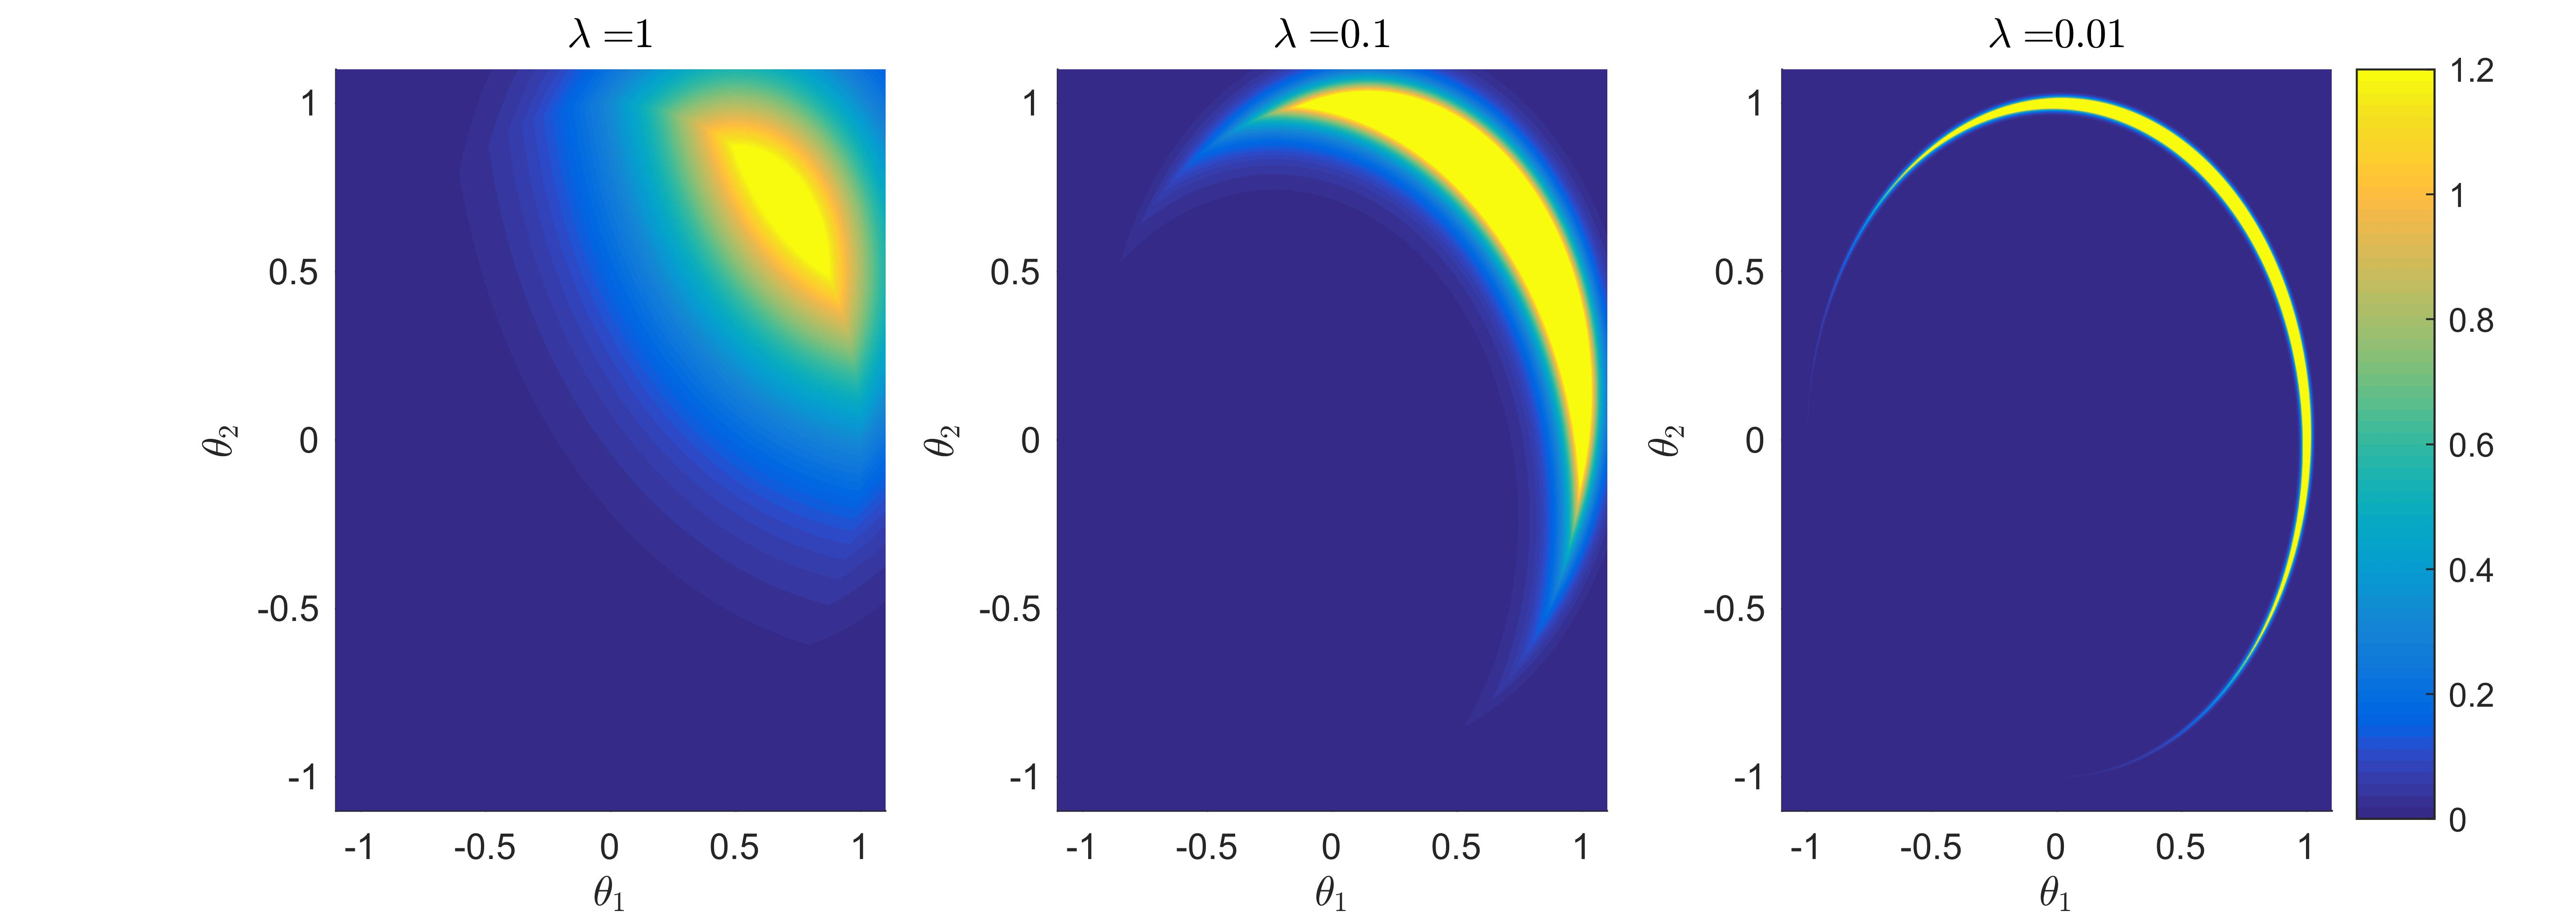
\includegraphics[width=1\textwidth]{Bivariate_Normal_Unit_Circle_Constraint}
% \caption{The relaxed distribution from a von Mises--Fisher
% distribution $\mbox{vMF}(
% [1/\sqrt{2},1/\sqrt{2}]',1/25)$. With decreasing
% $\lambda$, the relaxation is reduced and the circular
% constraint becomes clear.}
% \label{FIG:Bivariate_Normal_Unit_Circle_Constraint}
% \end{center}
% \end{figure}


\end{document}


